% *********************************************************************
% © 2021–2024 Jeremy Sylvestre
%
% Permission is granted to copy, distribute and/or modify this document
% under the terms of the GNU Free Documentation License, Version 1.3 or
% any later version published by the Free Software Foundation; with no
% Invariant Sections, no Front-Cover Texts, and no Back-Cover Texts. A
% copy of the license is included in the appendix entitled “GNU Free
% Documentation License” that appears in the output document of this
% PreTeXt source code. All trademarks™ are the registered® marks of
% their respective owners.
%
% *********************************************************************

\newcommand*{\xmin}{-0.25}
\newcommand*{\xmax}{7}
\newcommand*{\ymin}{-1.25}
\newcommand*{\ymax}{1.25}

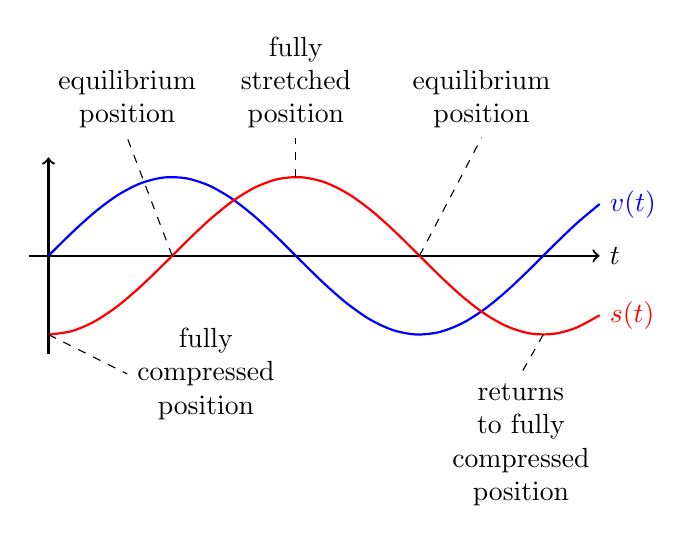
\begin{tikzpicture}
[
	closedpt/.style={circle,draw,fill,inner sep=0pt,minimum size=4pt},
	openpt/.style={circle,draw,inner sep=0pt,minimum size=4pt}
]

	% axes
	\draw[->,thick] (\xmin,0) -- (\xmax,0) node[right] {$t$};
	\draw[->,thick] (0,\ymin) -- (0,\ymax); % node[right] {$v(t)$};

	\draw[blue,thick,domain=0:\xmax,smooth] plot (\x,{sin(deg(\x))})
		node[right] {$v(t)$};

	\draw[red,thick,domain=0:\xmax,smooth] plot (\x,{- cos(deg(\x))})
		node[right] {$s(t)$};

	\draw[dashed] (0,-1) -- (1,-1.5) node[right, text width=1.75cm, align=center] {fully compressed position};

	\draw[dashed] (1.571,0) -- (1,1.5) node[above, text width=1.75cm, align=center] {equilibrium position};

	\draw[dashed] (3.142,1) -- (3.142,1.5) node[above, text width=1.5cm, align=center] {fully stretched position};

	\draw[dashed] (4.712,0) -- (5.5,1.5) node[above, text width=1.75cm, align=center] {equilibrium position};

	\draw[dashed] (6.284,-1) -- (6,-1.5) node[below, text width=2cm, align=center] {returns to fully compressed position};

\end{tikzpicture}
